\chap{Bipolar Junction Transistor}
\section{Introduction}
In the diode tutorials we saw that simple diodes are made up from two pieces of semiconductor material to form a simple pn-junction and we also learnt about their properties and characteristics.\\

\begin{figure}[!htp]
    \centering
    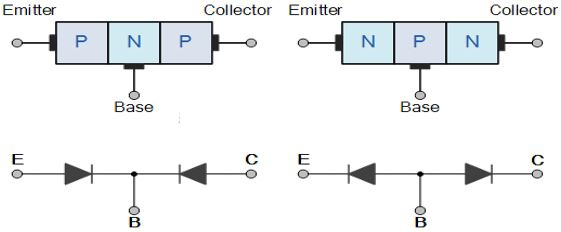
\includegraphics[width=4in]{source/picture/bai_3/BJT_1.jpg}
    \caption{\textit{Bipolar transistor construction}}
    \label{bai3_pic1}
\end{figure}

If two individual signal diodes are joined together back-to-back, this will form a two PN-junctions connected together in series which would share a common Positive, (P) or Negative, (N) terminal. The fusion of these two diodes produces a three layer, two junction, three terminal device forming the basis of a Bipolar Junction Transistor (BJT), which is shown in the figure above.\\

Considering the symbol of the transistor in the schematic, the direction of the arrow always points from the positive P-type region to the negative N-type region for both transistor types, exactly the same as for the standard diode symbol.\\

The transistor is ability to change between these two states enables it to have two basic functions: “switching” (digital electronics) or “amplification” (analogue electronics). Then bipolar transistors have the ability to operate within three different regions:
\begin{itemize}
    \item Active region: The transistor operates as an amplifier and $I_C = \beta I_B$
    \item Saturation: The transistor is “Fully-ON” operating as a switch and $I_C = I_{Sat}$
    \item Cut-off: The transistor is “Fully-OFF” operating as a switch and $I_C = 0$
\end{itemize}

\newpage
\section{BJT simulation circuit}
Implement the following circuit in PSPICE. The new component used is \textbf{QBreakN NPN}, which can be found in the Favorites list. The default transistor gain is $\beta = 100$, and the saturated voltage $V_{CE(Sat)} = 0.65V$

\begin{figure}[!htp]
    \centering
    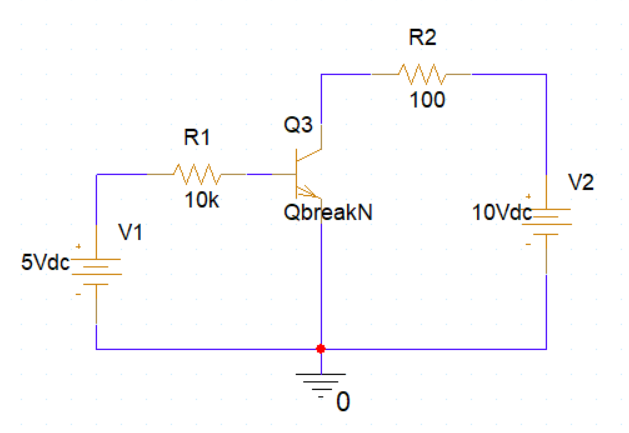
\includegraphics[width=4in]{source/picture/bai_3/manual_pic1.PNG}
    \caption{\textit{Simple connection with transistor}}
    \label{bai3_manual_1}
\end{figure}

For a bias point simulation profile, the following results are expected: 

\begin{figure}[!htp]
    \centering
    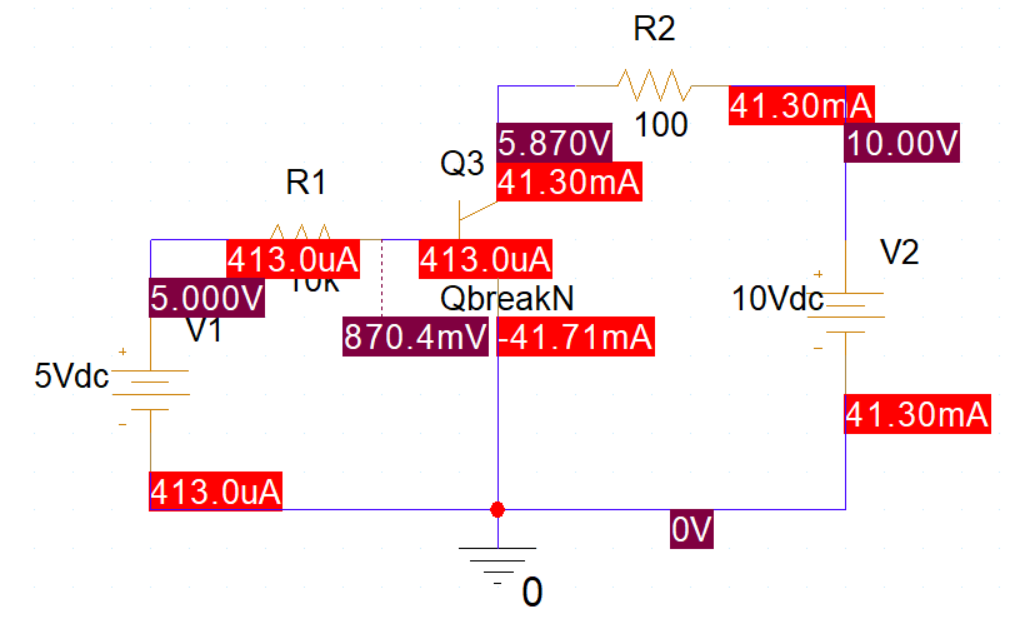
\includegraphics[width=4in]{source/picture/bai_3/manual_pic2.PNG}
    \caption{\textit{Bias profile simulation results}}
    \label{bai3_manual_2}
\end{figure}

It is assumed that $V_{BE} = 0.7V$, the simulation results in PSPice are explained as follows:
\begin{itemize}
    \item According to the Ohm Low, $I_B = (V_{BB} - V_{BE})/R1$ = (5V - 0.7V)/10k = 0.43mA
    \item It is assumed that the transistor is in linear (or active) mode, $I_C = \beta * I_B$ = 43mA
    \item Finally, in order to confirm the assumption above, $V_{CE} = V_{CC} - I_C*R2$ = 10V - 43mA * 100Ohm = 5.7V
\end{itemize}

Since $V_{CE} > V_{CE(Sat)}$, the transistor is working in the linear mode, to confirm our assumption. Moreover, the theory calculation is very close to the PSpice simulations.

\section{Exercise and Report}
\subsection{BJT in Saturation Mode}
Change the value of \textbf{R1 to 1k} and run the simulation again. Capture the simulation results and explain the values of $I_B, I_C, V_{CE}$. The default transistor gain is $\beta = 100$, and the saturated voltage $V_{CE(Sat)} = 0.65V$ and $V_{BE} = 0.7V$.


\textbf{\textit{Your image goes here:}}\\
\vspace{6cm}

The results in PSpice are explained as follows:

\begin{itemize}
    \item According to the Ohm Low, $I_B =$ \dotfill
    \item It is assumed that the transistor is in linear (or active) mode, $I_C = \beta * I_B$ = \dotfill
    \item Finally, in order to confirm the assumption above, $V_{CE} = V_{CC} - I_C*R2$ = \dotfill
\end{itemize}

Since $V_{CE} < 0$, our assumption is not correct. The transistor stays in saturation mode. Therefore, $I_C$ is determined as follows:\\

$I_C = (V_{CC} - V_{CE(Sat)}) / R2$ = \dotfill\\

\newpage
\subsection{DC Sweep Simulation}
The schematic in the first exersice with \textbf{R1 = 1k} is re-used in this exercise. However, a DC-Sweep simulation mode is performed with V1 is varied from 0V to 5V (0.1V for the step), as follows:

\begin{figure}[!htp]
    \centering
    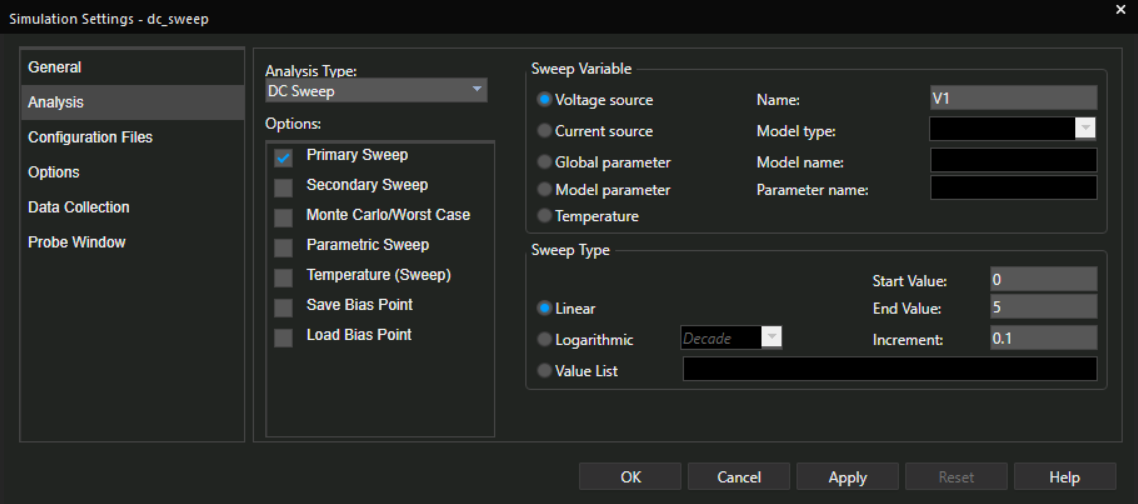
\includegraphics[width=4in]{source/picture/bai_3/dc_sweep_simul.PNG}
    \caption{\textit{DC-Sweep profile for simulation}}
    \label{bai3_manual_2}
\end{figure}

Run the simulation and trace for the current $I_C$ according to the value of V1. Capture your screen and plot it in the report. Please increase the width of the curve.

\textbf{\textit{Your image goes here:}}\\
\vspace{6cm}


When the transistor becomes saturation, the value of V1 is \dotfill\bigskip\\
At this value, the value of $I_B$ is \dotfill\bigskip\\
And the value of $I_{C(Sat)}$ is \dotfill\bigskip\\


\subsection{BJT used as a Switch}
For a given BJT circuit, determine R1 and R2 to have IC saturated at 50mA. In this saturation mode, $V_{CE(Sat)}$ is 30mV. Assume that $V_{BE}$ = 0.7V and the current gain $\beta$ = 100.

\newpage
\begin{figure}[!htp]
    \centering
    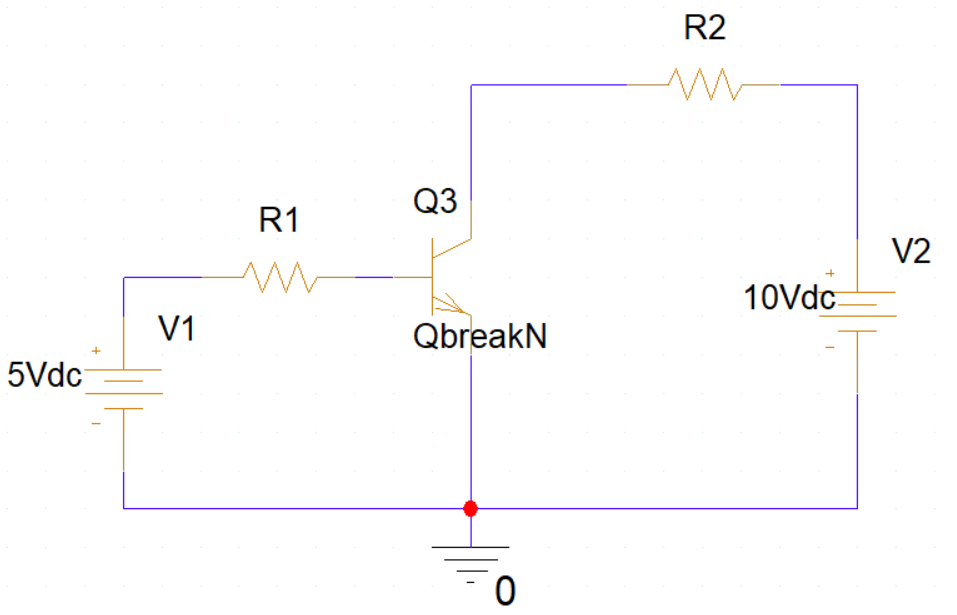
\includegraphics[width=4in]{source/picture/bai_3/pic2.PNG}
    \caption{\textit{BJT used as switch in saturation mode}}
    \label{bai3_manual_2}
\end{figure}


Present your solution to determine R1 and R2.
Perform the simulation in PSpice to confirm the results. Capture the screen in PSpice and present in the report.\\




\textbf{\textit{Your image goes here:}}\\
\vspace{6cm}


\subsection{Drive a device with an NPN BJT}
This exercise has a $5V$ logic output (the $V_{ter}$ in Figure \ref{lab3_ex2_de}) that can source up to $10mA$ of current without a severe voltage drop and stand a maximum current of $20mA$. If the logic terminal sources a current larger than $20mA$, it would be damaged. Or, if it sources a current larger than $10mA$, the $V_{ter}$ voltage will drop to less than $4V$. We should avoid this drop in many cases.  However, this logic terminal has to be used to drive an electrical component with an equivalent internal resistance of 5 ohms (the LOAD in Figure \ref{lab3_ex2_de}) and requires a current of at least $300mA$ and not exceeding $500mA$ to function normally.
Given that we have an NPN transistor with the current gain $\beta$ equals $100$, the maximum $I_C$ current is $400mA$, and the barrier potential at the BE junction is $V_{BE} = 0.7V$, select a resistor available in the market to replace the resistor $R_B$ revealed in Figure \ref{lab3_ex2_de}. to make the circuit function well. After that, perform a simulation to double-check your selection.

\begin{figure}[H]
    \centering
    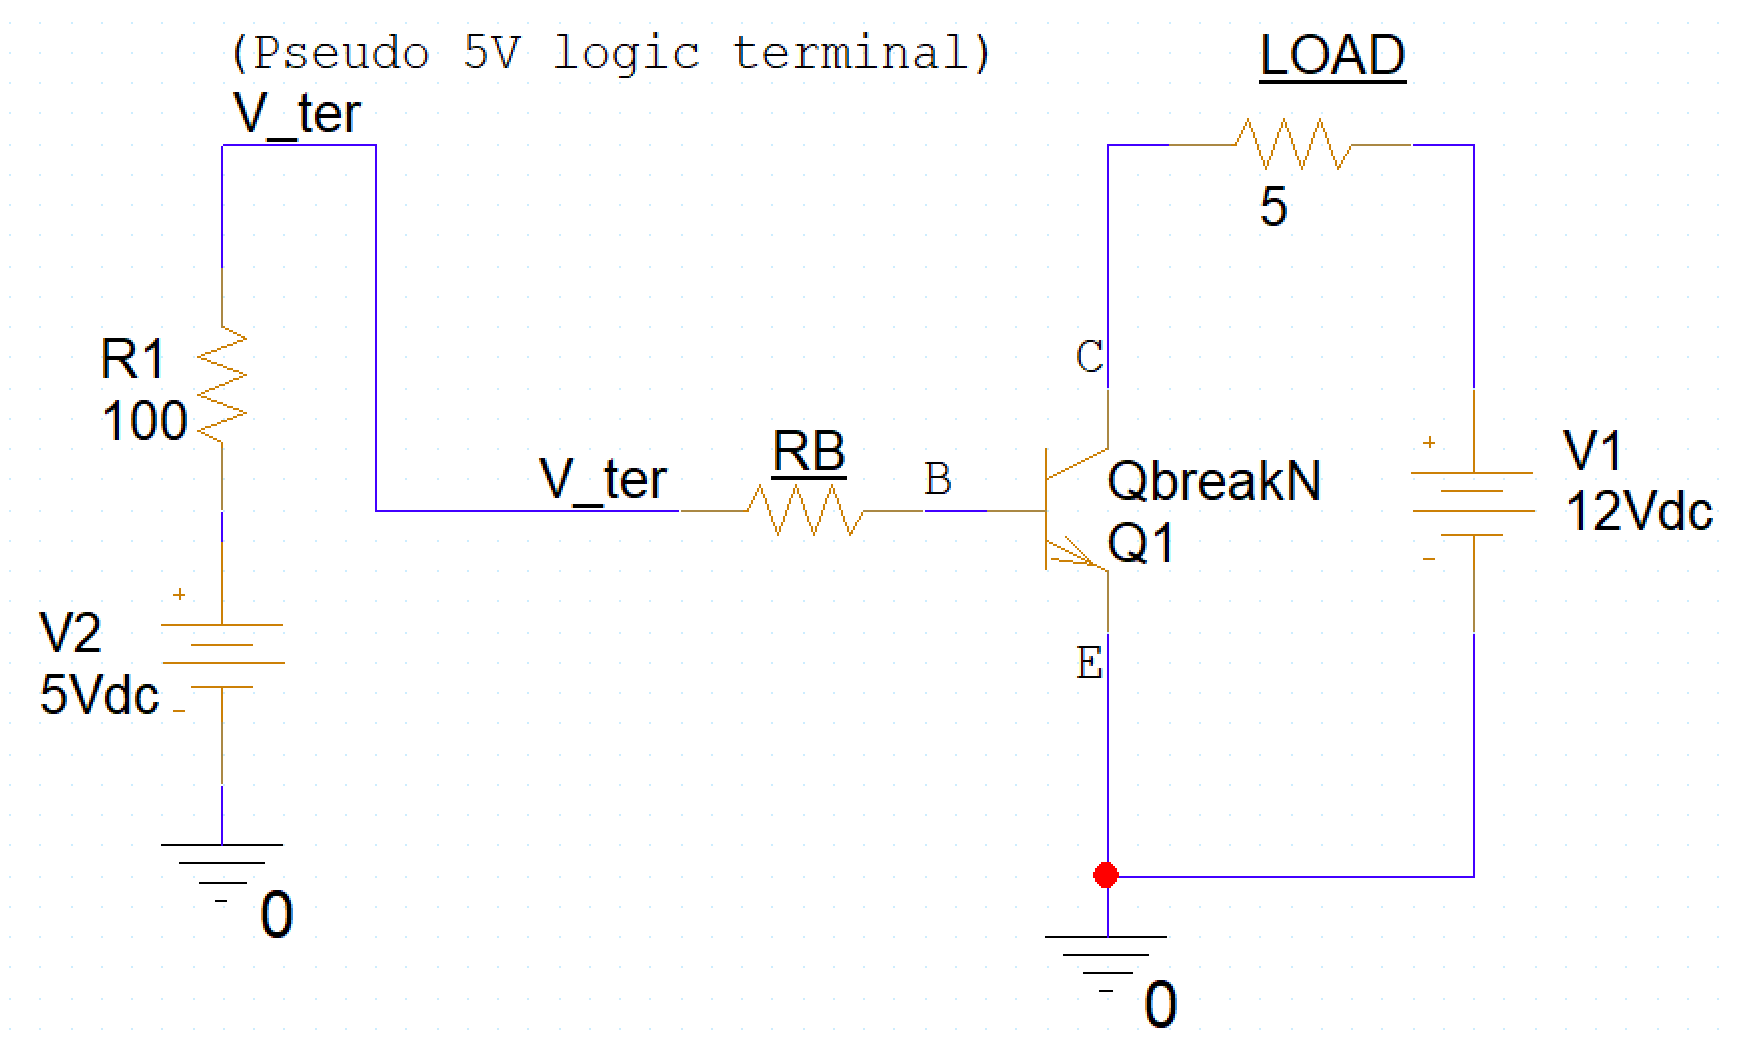
\includegraphics[width=12cm]{source/picture/bai_3/lab3_ex2_de.png}
    \caption{Select a resistor available in the market for $R_B$}
    \label{lab3_ex2_de}
\end{figure}

\subsubsection{Theory calculations}
\textit{\textbf{Notes:}}\\
\textit{Explanations, formulas, and equations are expected rather than only results.}\\
\\
According to the limits of the LOAD and the transistor, we have:\bigskip\\
\begin{center}
    \dotfill (min) $< I_C <$\dotfill(max)\bigskip\\
    \dotfill (min) $< I_B <$\dotfill(max)\bigskip\\
    With $I_B(min) = $\dotfill we have:\bigskip\\
    $R_B(max) = $\dotfill\bigskip\\
    With $I_B(max) = $\dotfill we have:\bigskip\\
    $R_B(min) = $\dotfill\bigskip\\
\end{center}

So:\bigskip

\begin{center}
    \dotfill (min) $< R_B <$\dotfill(max)\bigskip\\
    $R_B$ selected:\dotfill\bigskip\\
\end{center}


\subsubsection{Simulation}
\textbf{\textit{Your image goes here}}
\vspace{8cm}

\subsubsection{Compare}
\begin{center}
    \begin{tabular}{l|l|l|l|l|l|l|l|}
    \cline{2-8}
                                     & & \multicolumn{3}{c|}{\textbf{Theory}} & \multicolumn{3}{c|}{\textbf{PSpice}} \\ \cline{2-8} 
                                     &$R_B$ & $V_{BE}$              & $I_B$              & $I_C$              & $V_{BE}$              & $I_B$              & $I_C$             \\ \hline
     \multicolumn{1}{|l|}{$R_B(min)$} &      &          &                &                &                &                &               \\ \hline
    \multicolumn{1}{|l|}{$R_B(max)$}  &        &        &                &                &                &                &               \\ \hline
        \multicolumn{1}{|l|}{$R_B(selected)$}  &       &         &                &                &                &                &               \\ \hline

    \end{tabular}
\end{center}


\subsection{Simple bias configuration}
The circuit given in Figure \ref{lab3_ex5_de} is known as a simple kind of NPN bias configuration. First, students simulate the circuit with two values of RC, respectively 10 Ohms and 1k Ohms. Then, give your statement on the change of the current $I_E$ and explain the phenomena.

\begin{figure}[H]
    \centering
    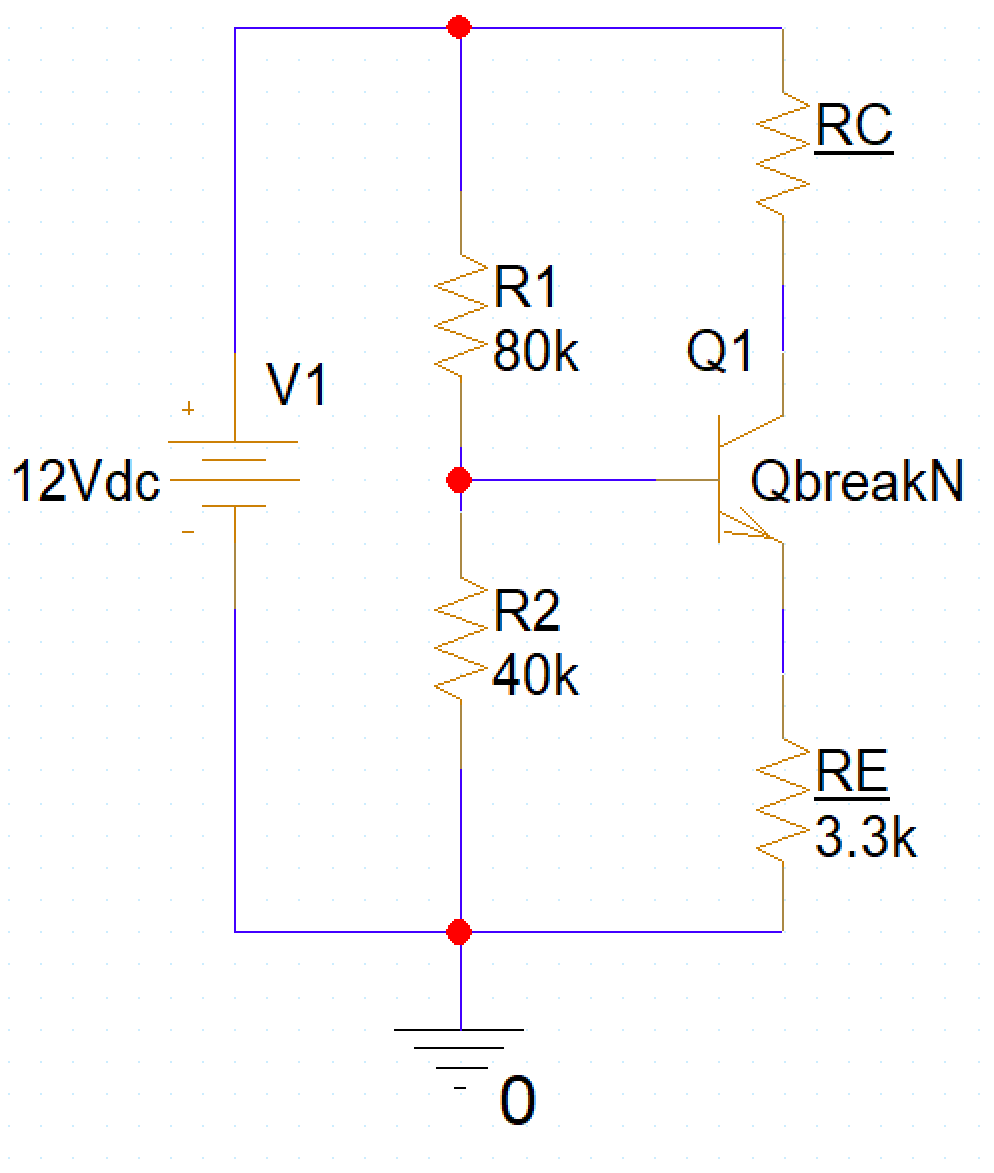
\includegraphics[width=8cm]{source/picture/bai_3/lab3_ex5_de.png}
    \caption{Simple bias configuration}
    \label{lab3_ex5_de}
\end{figure}

\subsubsection{Simulation}
\textbf{\textit{Your images go here (2 images)}}\\
\textbf{\textit{Step 1}}: Simulate the circuit with $R_C$ = 10 Ohms.\\
\textbf{\textit{Step 2}}: Simulate the circuit with $R_C$ = 1k Ohms.
\vspace{8cm}\\

\subsubsection{Circuit analysis}
Conduct some theoretical calculation to explain for the phenomena you have observed from the simulation. \bigskip\\

\dotfill\bigskip\par\mbox{}\dotfill
\dotfill\bigskip\par\mbox{}\dotfill
\dotfill\bigskip\par\mbox{}\dotfill
\dotfill\bigskip\par\mbox{}\dotfill
\dotfill\bigskip\par\mbox{}\dotfill
\dotfill\bigskip\par\mbox{}\dotfill
\dotfill\bigskip\par\mbox{}\dotfill
\dotfill\bigskip\par\mbox{}\dotfill



\subsection{PNP Circuit}
Figure \ref{lab3_ex6_de} shows a very typical PNP transistor circuit.
Calculate $I_B$, $I_E$, and $I_C$ then simulate the circuit to double-check your calculation. Assume the current gain $\beta$ = 100.

\begin{figure}[H]
    \centering
    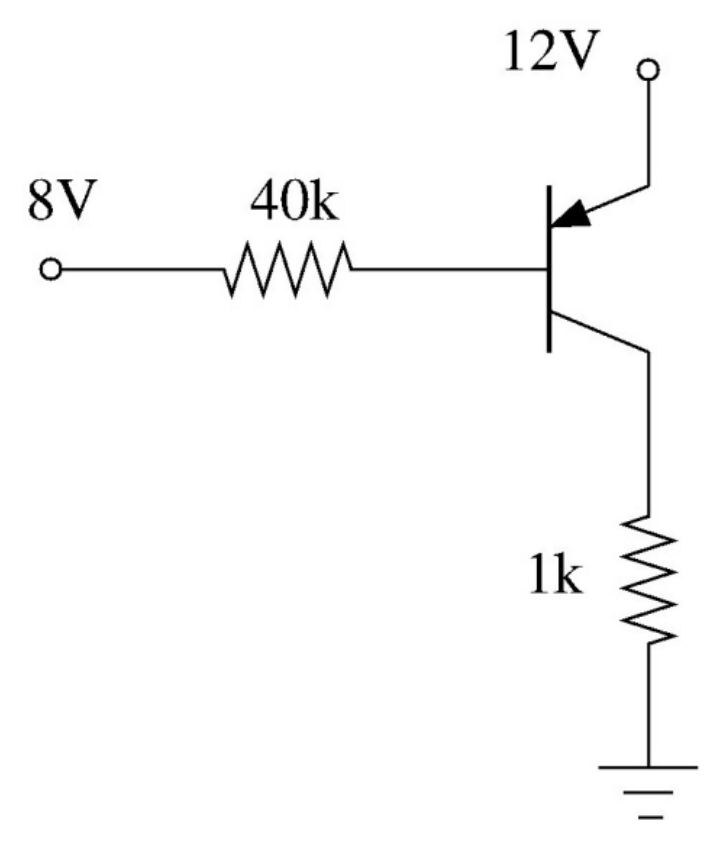
\includegraphics[width=6cm]{source/picture/bai_3/lab3_ex6_de.png}
    \caption{A PNP Circuit}
    \label{lab3_ex6_de}
\end{figure}

\subsubsection{Theoretical calculation}
\textit{\textbf{Notes:}}\\
\textit{Explanations, formulas, and equations are expected rather than only results.}
\bigskip\\

$V_{EB}$ = \dotfill\bigskip\\
$I_B$ = \dotfill\bigskip\\
$I_C$ = \dotfill\bigskip\\
$I_E$ = \dotfill\bigskip\\

\subsubsection{Simulation}
\textbf{\textit{Your image goes here}}
\vspace{8cm}

\subsubsection{Comparison}
$I_B$ (In theory) = \dotfill $I_B$ (simulation) = \dotfill\bigskip\\
$I_C$ (In theory) = \dotfill $I_C$ (simulation) = \dotfill\bigskip\\
$I_E$ (In theory) = \dotfill $I_E$ (simulation) = \dotfill\bigskip\\


\subsection{Circuit with NPN and PNP bipolar junction transistors}
Give the circuit in Figure \ref{lab3_ex7_de}. Calculate the Voltage at all nodes and the current in all branches.
Assume the current gain of both transistors is the same at $\beta$ = 100. Then perform a simulation and compare the result with the theoretical calculation.

\begin{figure}[H]
    \centering
    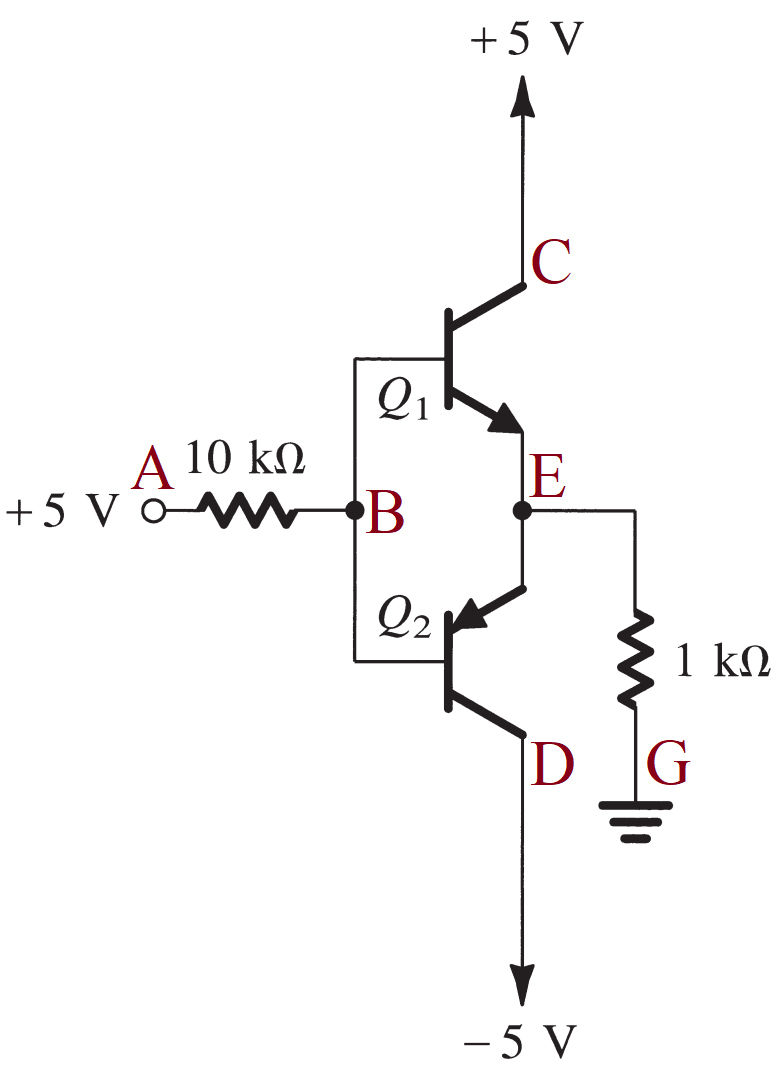
\includegraphics[width=6cm]{source/picture/bai_3/lab3_ex7_de.png}
    \caption{Circuit with NPN and PNP bipolar junction transistors}
    \label{lab3_ex7_de}
\end{figure}

\subsubsection{Theoretical calculation}
\textit{\textbf{Notes:}}\\
\textit{Explanations, formulas, and equations are expected rather than only results.}
\bigskip\\
We have $V_E$ (compare to)\dotfill $V_B$, therefore the transistor $Q_2$ is \dotfill\\
According to the \dotfill, we have the following equation:\bigskip\\
$I_{BE}$ (hereinafter called $I_B$) = \dotfill (1)\bigskip\\
Solve (1) we have $I_B$ = \dotfill\bigskip\\
$I_C$ = \dotfill\bigskip\\
$I_{EG}$ = \dotfill\bigskip\\
$V_E$ = \dotfill\bigskip\\
$V_B$ = \dotfill\bigskip\\

\subsubsection{Simulation}
\textbf{\textit{Your image goes here}}
\vspace{8cm}

\subsubsection{Comparison}
$I_B$ (In theory) = \dotfill $I_B$ (simulation) = \dotfill\bigskip\\
$I_C$ (In theory) = \dotfill $I_C$ (simulation) = \dotfill\bigskip\\
$I_{EG}$ (In theory) = \dotfill $I_{EG}$ (simulation) = \dotfill\bigskip\\
$V_E$ (In theory) = \dotfill $V_E$ (simulation) = \dotfill\bigskip\\
$V_B$ (In theory) = \dotfill $V_B$ (simulation) = \dotfill\bigskip\\

\subsection{NPN Circuit with E resistance}
In Figure \ref{lab3_ex9_de}, calculate all the values of $I_B$, $I_C$, $I_E$, $V_E$, and $V_C$. Assume the voltage drop $V_{BE}$ = 0.7V and the current gain coefficient of the transistor is $\beta$ = 100. Then, perform a simulation to double-check your theoretical calculations.

\begin{figure}[H]
    \centering
    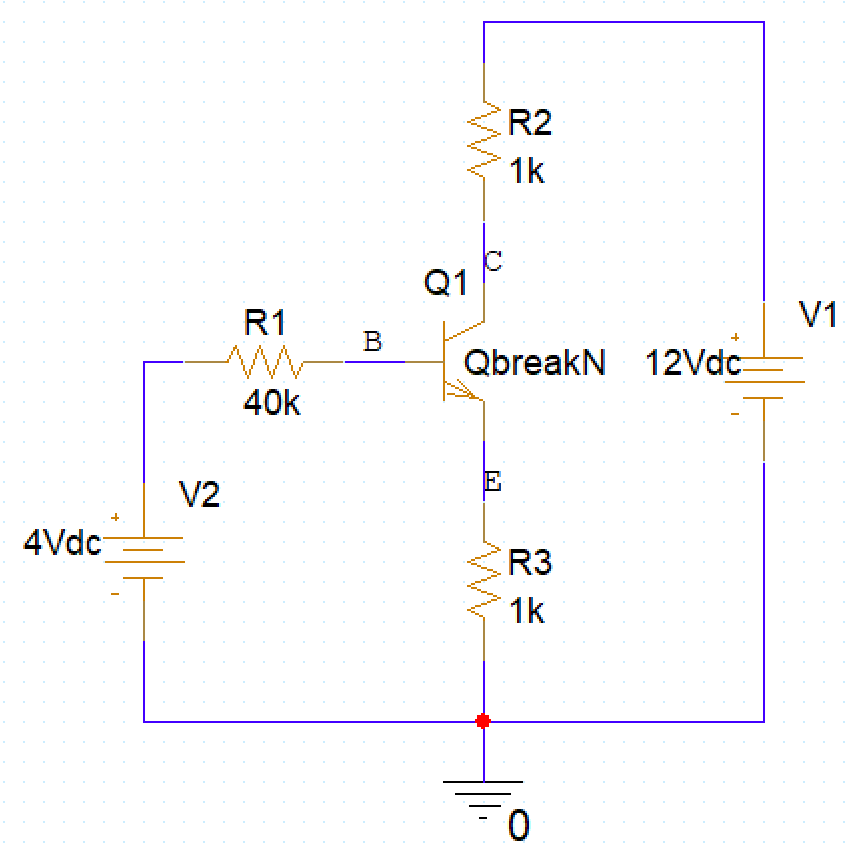
\includegraphics[width=10cm]{source/picture/bai_3/lab3_ex9_de.png}
    \caption{NPN Circuit with E resistance}
    \label{lab3_ex9_de}
\end{figure}

\subsubsection{Theoretical calculation}
\textit{\textbf{Notes:}}\\
\textit{Explanations, formulas, and equations are expected rather than only results.}
\bigskip\\

According to the \dotfill, we have the following equation:\bigskip\\
\dotfill\bigskip\par\mbox{}\dotfill\bigskip\\
$\iff$\dotfill (1)\bigskip \\
Solve (1), we have $I_B$ = \dotfill\bigskip\\
$I_C$ = \dotfill\bigskip\\
$I_E$ = \dotfill \bigskip\\
$V_E$ = \dotfill \bigskip \\
$V_C$ = \dotfill \bigskip \\

\subsubsection{Simulation}
\textbf{\textit{Your image goes here}}
\vspace{8cm}


\subsection{Darlington circuit}
The circuit given in Figure \ref{lab3_ex8_de} is known as a darlington circuit.
Calculate $I_{BE}$, $I_{AC}$, $I_{AL}$, and the overall current gain $\frac{I_{AL}}{I_{BE}}$. After that, simulate the circuit to double-check your theoretical calculations. Assume both transistors have the same current gain coefficient $\beta$ = 100.

\begin{figure}[H]
    \centering
    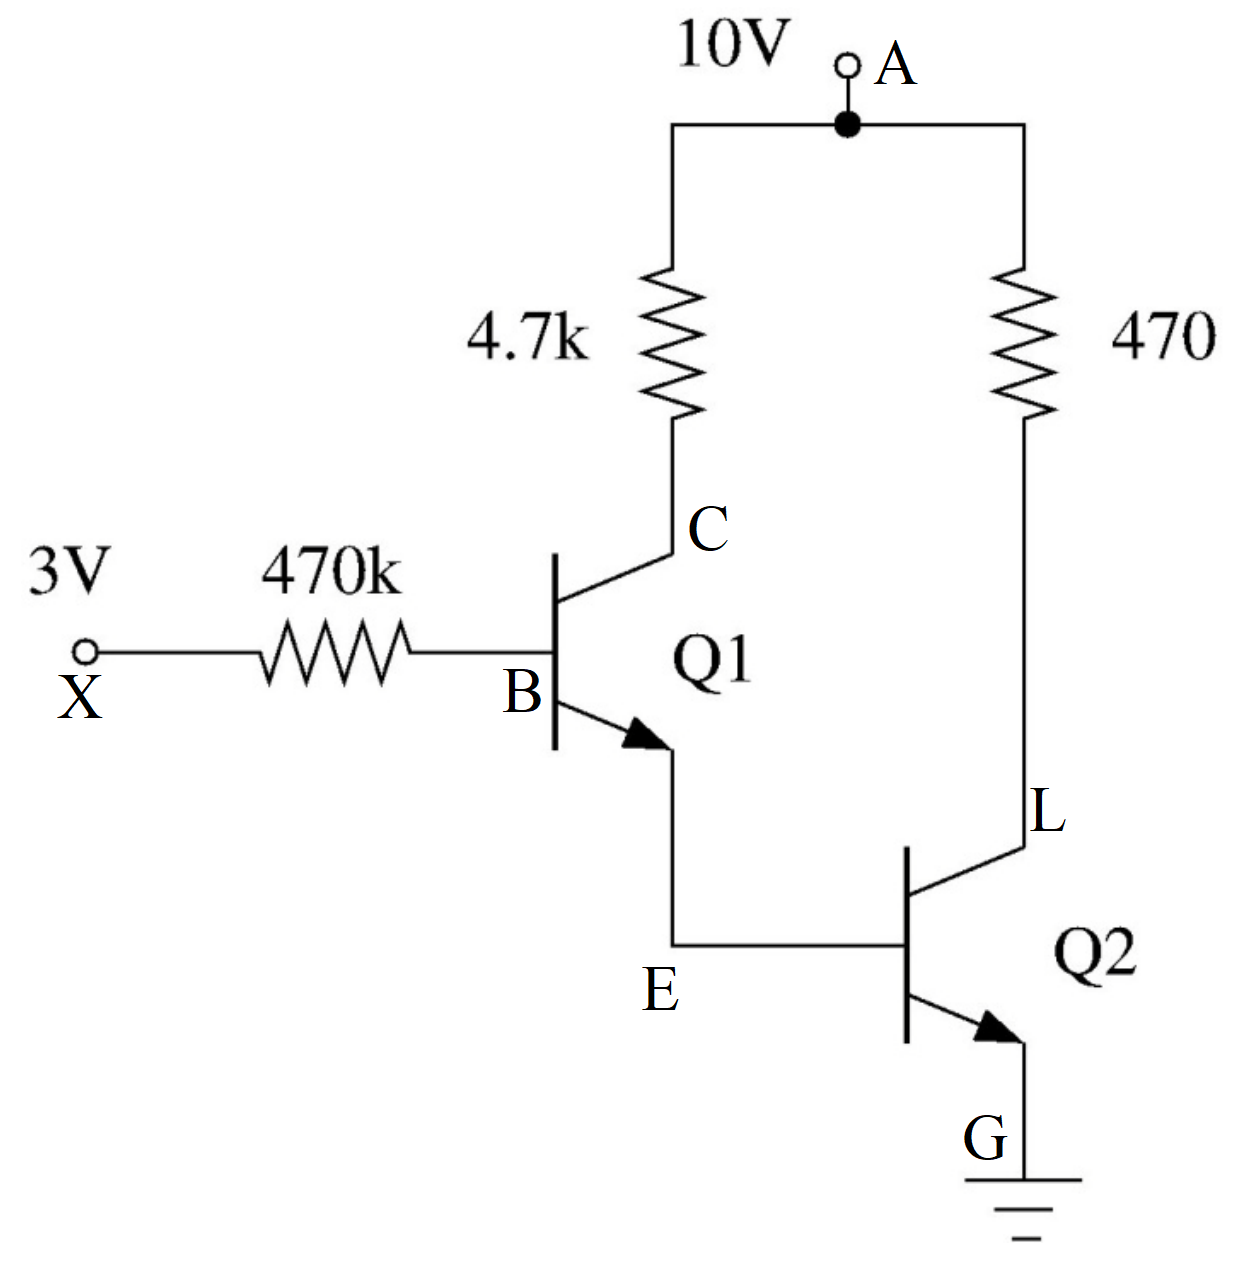
\includegraphics[width=8cm]{source/picture/bai_3/lab3_ex8_de.png}
    \caption{Darlington circuit}
    \label{lab3_ex8_de}
\end{figure}

\subsubsection{Theoretical calculation}
\textit{\textbf{Notes:}}\\
\textit{Explanations, formulas, and equations are expected rather than only results.}
\bigskip\\

$I_{BE}$ = \dotfill\bigskip\\
$I_{AC}$ = \dotfill\bigskip\\
$I_{AL}$ = \dotfill\bigskip\\
$\frac{I_{AL}}{I_{BE}}$ = \dotfill\bigskip\\

\newpage

\subsubsection{Simulation}
\textbf{\textit{Your image goes here}}
\vspace{8cm}
\\

\subsection{Common base}

Figure \ref{lab3_commonB_de} shows a bias techniques named common base bias.
Calculate the values of $I_E$, $I_B$, $I_C$, and $V_{CE}$. Then simulate the circuit to double-check your theoretical calculations. Assume the current gain coefficient $\beta$ = 100.

\begin{figure}[H]
    \centering
    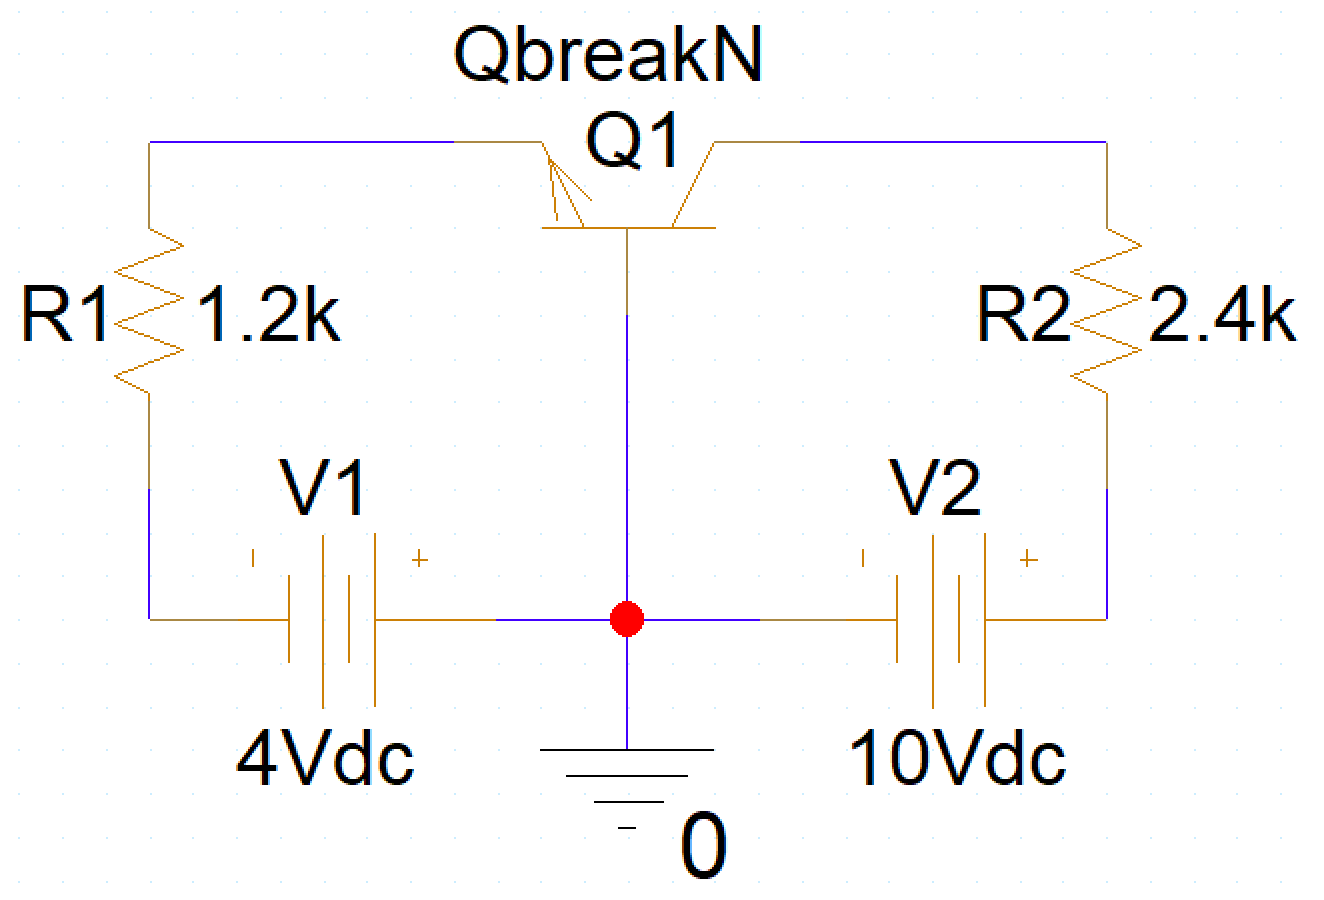
\includegraphics[width=8cm]{source/picture/bai_3/lab3_commonBase_de.png}
    \caption{Common base}
    \label{lab3_commonB_de}
\end{figure}

\subsubsection{Theoretical calculation}
\textit{\textbf{Notes:}}\\
\textit{Explanations, formulas, and equations are expected rather than only results.}
\bigskip\\
According to the \dotfill we have: \bigskip\\
$I_E$ = \dotfill\bigskip\\
$I_B$ = \dotfill\bigskip\\
$I_C$ = \dotfill\bigskip\\
$V{C_E}$ = \dotfill\bigskip\\

\subsubsection{Simulation}
\textbf{\textit{Your image goes here}}
\vspace{8cm}
\\

\subsection{Current mirror}
The circuit shown in Figure \ref{lab3_currentMirror_de} is known as a current mirror circuit. First, students do some theoretical calculations to get an understanding of it. After that, perform a simulation to double-check its principles and your analysis. Assume that the two transistors Q1 and Q2, are the same type and the current gain $\beta$ = 100.

\begin{figure}[H]
    \centering
    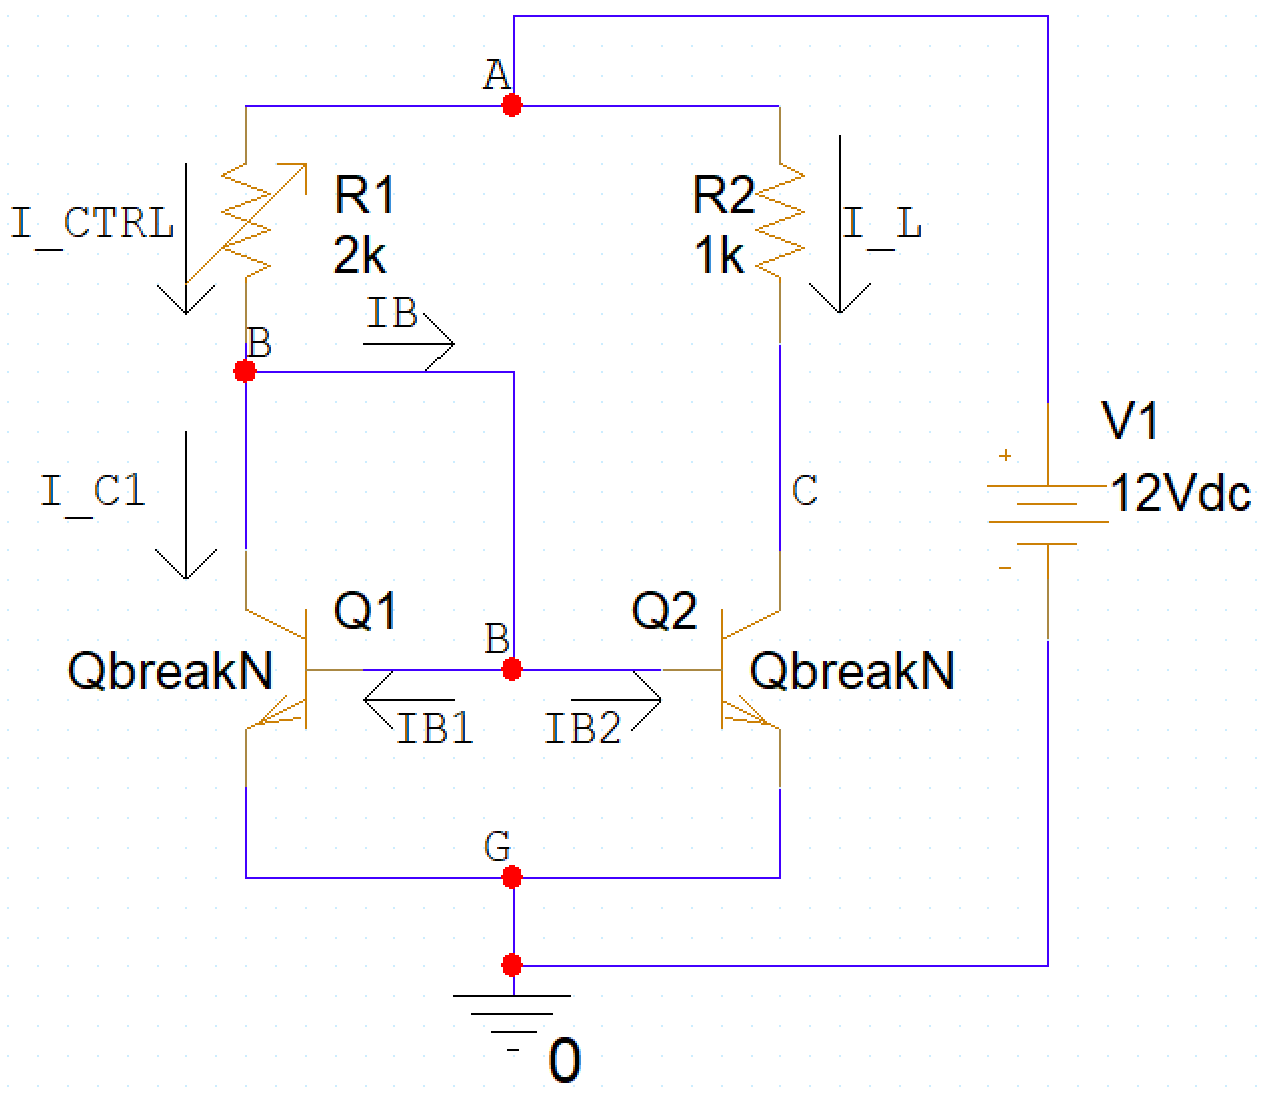
\includegraphics[width=9cm]{source/picture/bai_3/lab3_currenMirror_de.png}
    \caption{Current mirror circuit example}
    \label{lab3_currentMirror_de}
\end{figure}

\subsubsection{Theoretical calculation}
\textit{\textbf{Notes:}}\\
\textit{Explanations, formulas, and equations are expected rather than only results.}
\bigskip\\
According to the \dotfill we have: \bigskip\\
$I_{CTRL}$ = \dotfill \bigskip \\
$I_{C_1}$ = \dotfill \bigskip \\
$I_{B_1}$ = $I_{B_2}$ = \dotfill \bigskip \\
$I_L$ = \dotfill \bigskip \\

\subsubsection{Simulation}
\textbf{\textit{Your image goes here}}
\vspace{8cm}
\\
Why is the circuit in Figure \ref{lab3_currentMirror_de} called circuit mirror?
\dotfill\bigskip\par\mbox{}\dotfill\bigskip\\
Now, replace the resistor $R_1$ with a 100-Ohms one. Next, calculate all the values again. Then, finally, simulate the new circuit and explain the phenomena you've observed.\bigskip\\
$I_{CTRL}$ = \dotfill \bigskip \\
$I_{C_1}$ = \dotfill \bigskip \\
$I_{B_1}$ = $I_{B_2}$ = \dotfill \bigskip \\
$I_L$ = \dotfill \bigskip \\
\newpage
\textbf{\textit{The 2nd simulation result goes here}}:\\
\vspace{8cm}
\\
What is the phenomena? \bigskip\\
\dotfill\bigskip\par\mbox{}\dotfill\bigskip\\
\\
Explain:
\begin{center}
    \dotfill\bigskip\par\mbox{}\dotfill\bigskip\\
    \dotfill\bigskip\par\mbox{}\dotfill\bigskip\\
    \dotfill\bigskip\par\mbox{}\dotfill\bigskip\\
    \dotfill\bigskip\par\mbox{}\dotfill\bigskip\\
    \dotfill\bigskip\par\mbox{}\dotfill\bigskip\\
\end{center}

\subsection{BJT's logic gate application}
Figure \ref{lab3_notGate_de} describes a straightforward NOT gate theoretical implementation using an NPN bipolar junction transistor. In the circuit, the NPN junction transistor operates in the saturation mode.

\begin{figure}[H]
    \centering
    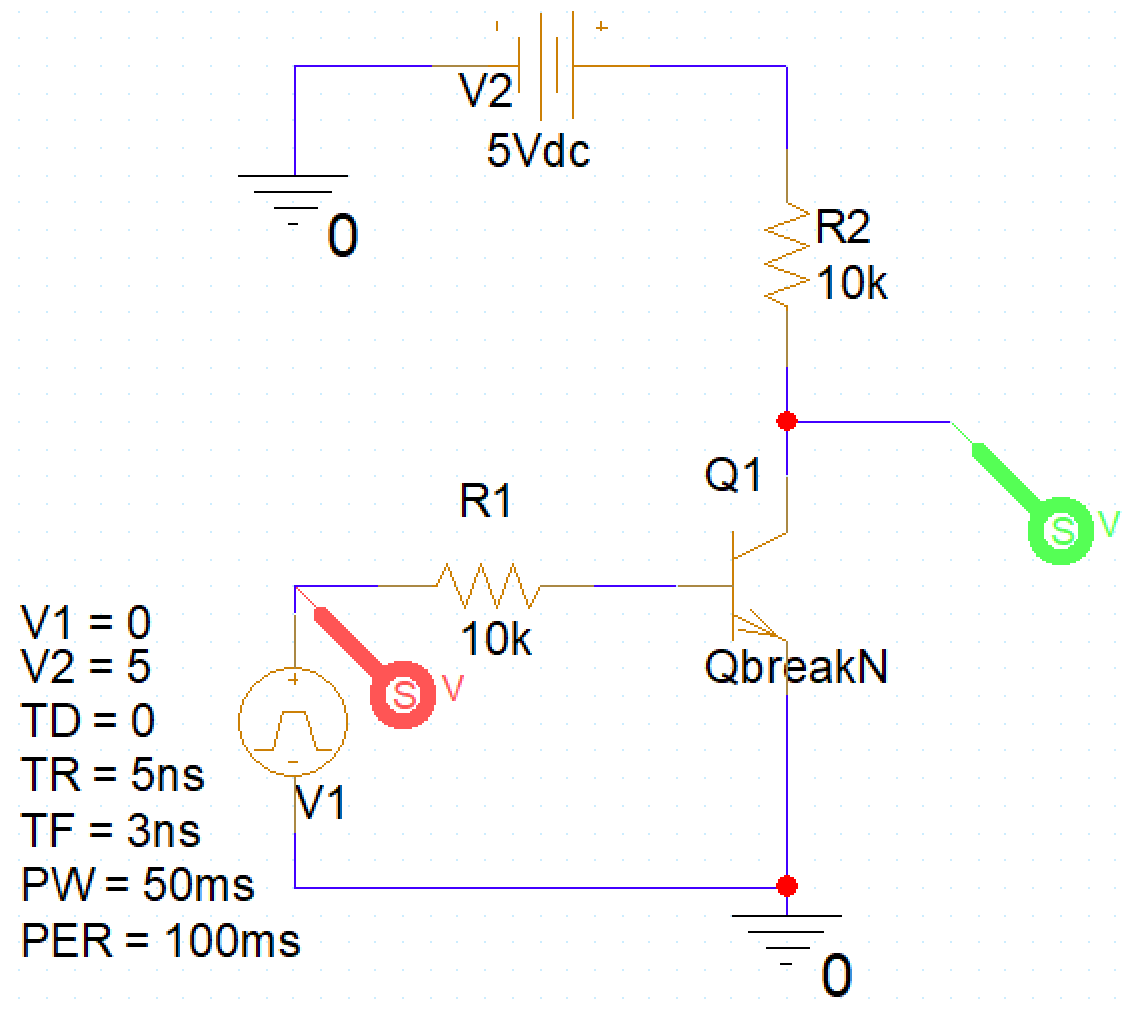
\includegraphics[width=10cm]{source/picture/bai_3/lab3_notGate_de.png}
    \caption{NPN theoretical NOT gate}
    \label{lab3_notGate_de}
\end{figure}

V1 = 0  When the source is off, the voltage would be 0V.\\
V2 = 5  When the source is on, the voltage would be 5V.\\
TD = 0  Delay time. This exercise assumes that there is no delay.\\
TR = 5ns  The rise time of the pulse (from off to on stage).\\
TF = 3ns  The fall time of the pulse (from on to off stage).\\
PW = 50ms  Pulse width: The time in which the source keeps on.\\
PER = 100ms  The period of the signal.\\

\textbf{\textit{Tips:}}\\
\\
To get the Voltage Pulse Source component in the PSpice for TI, go to \textbf{\textit{Place -> Pspice Compoment... -> Source -> Voltage Sources -> Pulse.}}

\newpage

\subsubsection{Simulation}
\textbf{\textit{Your image goes here}}\\
\vspace{8cm}
\\
But, wait! How large is the maximum current this NOT gate can source? Of course, it cannot exceed 5V/10kOhm. How tiny it is! So, what if we want to use it to drive an LED? Just put an additional 220 Ohm resistor in parallel with the existing 10k one. And in this case, the 10k resistor is quite useless. Therefore, in many cases, people let the collector pin of the transistor open. This design is called open-collector output, as shown in Figure \ref{lab3_openCollector_example}.

\begin{figure}[H]
    \centering
    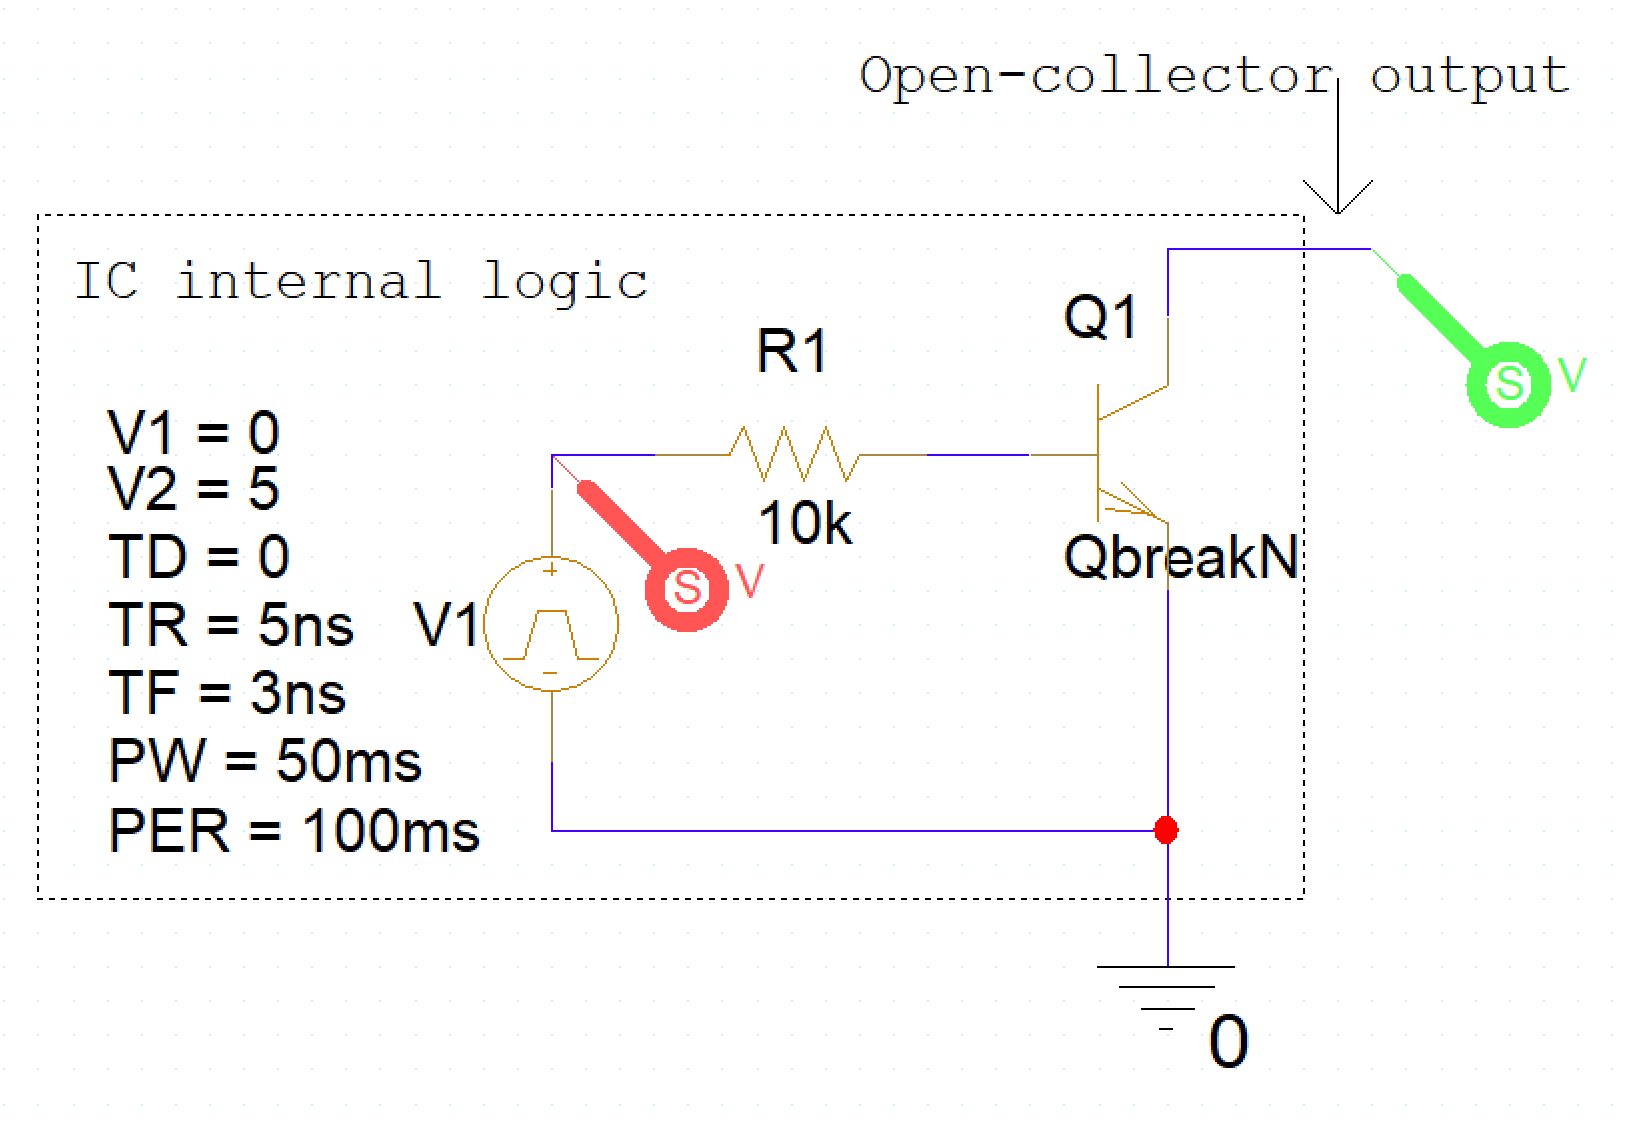
\includegraphics[width=12cm]{source/picture/bai_3/lab3_openCollector_example.png}
    \caption{Open-collector output example}
    \label{lab3_openCollector_example}
\end{figure}

But, with this design, the input of another IC can't read the voltage of this output. Because without a pull-up resistor, the voltage $V_C$ is floating. To read this voltage, the users have to pull it up using a resistor. There advantage here is to let the users choose the value of the pull-up resistor as their desire.

\begin{figure}[H]
    \centering
    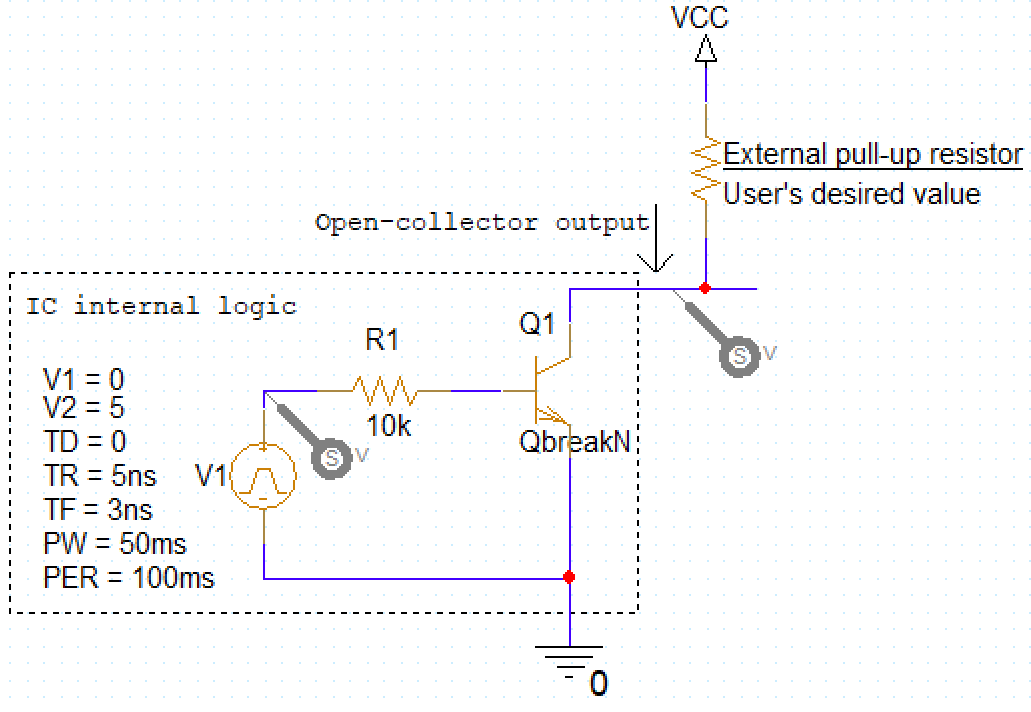
\includegraphics[width=15cm]{source/picture/bai_3/lab3_externalPullUp.png}
    \caption{External pull-up resistor whose value selected by the users}
    \label{lab3_externalPullUp}
\end{figure}

By the side, the open-collector design manner gives an exciting way of the use of these outputs, as shown in Figure \ref{lab3_wiredOC}. The open-collector wired output is at the LOW level if one of the elements is LOW and is HIGH only when all the elements output HIGH.

\begin{figure}[H]
    \centering
    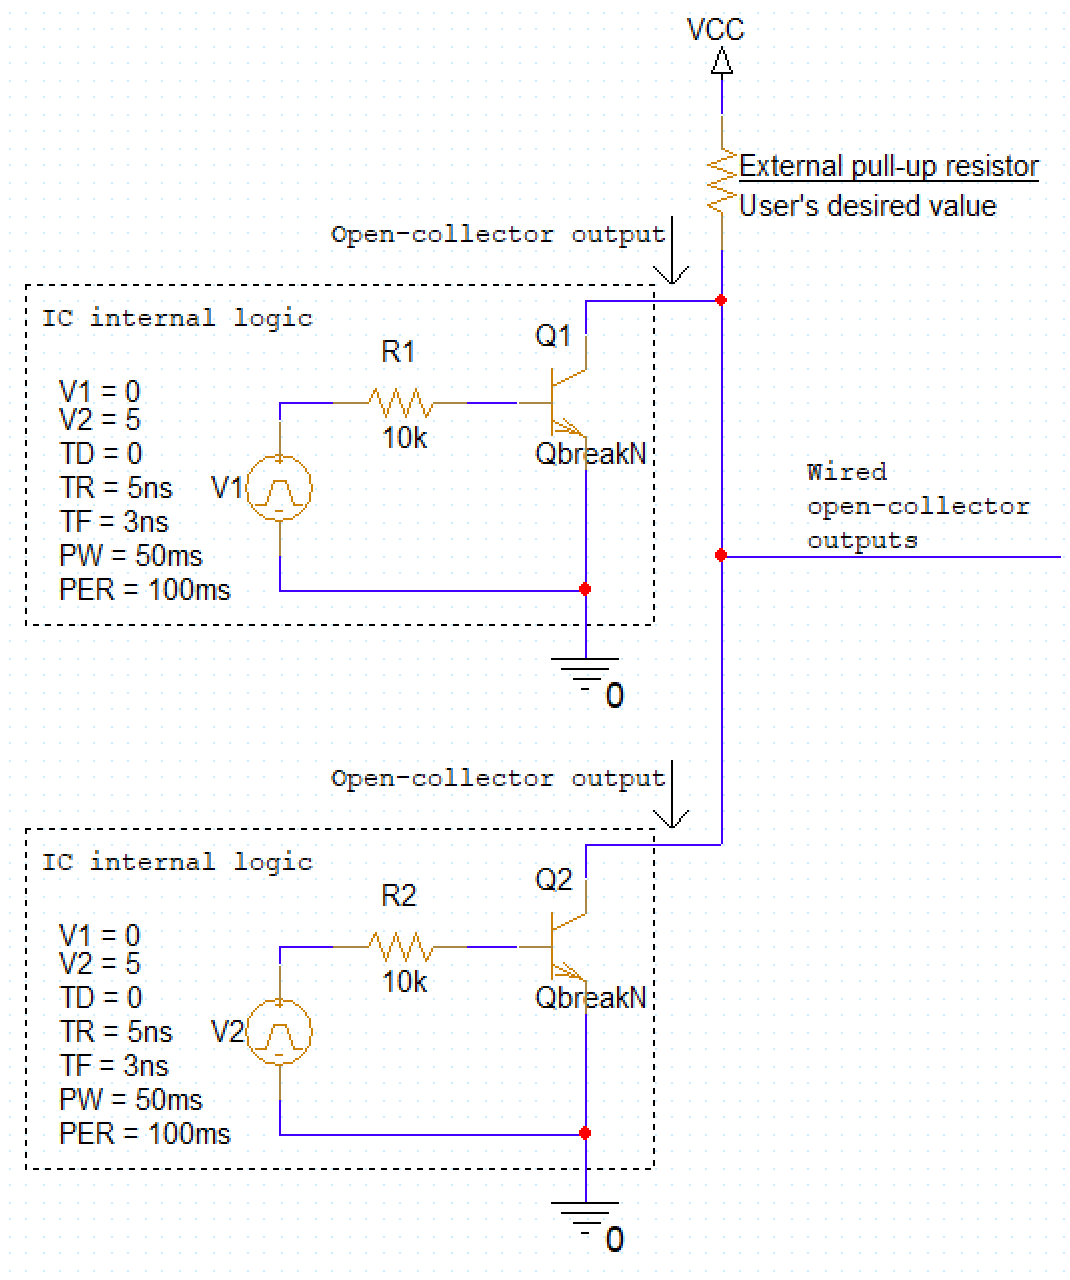
\includegraphics[width=15cm]{source/picture/bai_3/lab3_wiredOC.png}
    \caption{Wired open-collector outputs}
    \label{lab3_wiredOC}
\end{figure}

\subsection{Opto}

The element $OK_1$ in Figure \ref{lab3_opto_de} is an optocoupler, which includes a light-emitting diode (LED) and a photodiode. The photodiode's conductivity depends on the intensity of the light emitted by the LED, and of course, depends on the current intensity through the LED. When the voltage across the LED is lower than its barrier potential, the Opto is cut-off. When there is current through the LED, the Opto is in the transfer mode. Like the current gain $\beta$ of a BJT, the Opto also has the current transfer ratio (CTR). Assume the LED has its own barrier potential $V_F$ = 1.7V, and the Opto has the CTR = 2. Calculate the voltage $V_{OUT}$ when the switch is closed. Finally, give your idea about what we may use an Opto for, and how to use it? 


\begin{figure}[H]
    \centering
    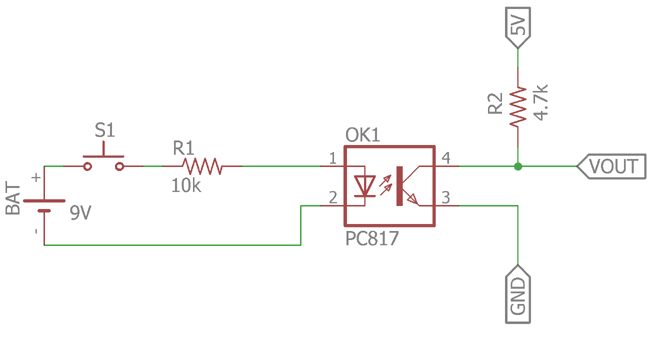
\includegraphics[width=12cm]{source/picture/bai_3/lab3_opto_de.png}
    \caption{Voltage isolation with opto}
    \label{lab3_opto_de}
\end{figure}

$I_F = I_{R_1}$ = \dotfill\bigskip\\
$I_{R_2}$ = \dotfill\bigskip\\
$V_{OUT}$ = \dotfill\bigskip\\
\begin{center}
    \dotfill\bigskip\par\mbox{}\dotfill\bigskip\\
    \dotfill\bigskip\par\mbox{}\dotfill\bigskip\\
    \dotfill\bigskip\par\mbox{}\dotfill\bigskip\\
    \dotfill\bigskip\par\mbox{}\dotfill\bigskip\\
    \dotfill\bigskip\par\mbox{}\dotfill\bigskip\\
\end{center}